\section{Scalability} \label{section:scalability}

From the runs shown in Figures \ref{fig:Spscale}, \ref{fig:Epscale}, and \ref{fig:kfscale}, it can be observed that the effectiveness of the developed solution improves with size, with the speedup from parallelising the implementation maximised for $n=2048$. For $n=256$ and $n=512$, Figure \ref{fig:Spscale} shows speedup gradually tapering off above $p\approx15$. This can be explained as past this point, the overhead of orchestrating the parallelisation outweighs the benefit gained from the parallelisation. For $n=1024$ and $n=2048$ however, the same cannot be said. Here, initial maxima in speedup are observed at $p\approx20$, and then again at $p\approx30$ for $n=1024$ and $p\approx35$ for $n=2048$. This implies that unlike for the two smaller matrices, the benefit of the parallelisation begins to outweigh the orchestration overhead for larger and larger $p$. 

\begin{figure}[H]
    \centering
    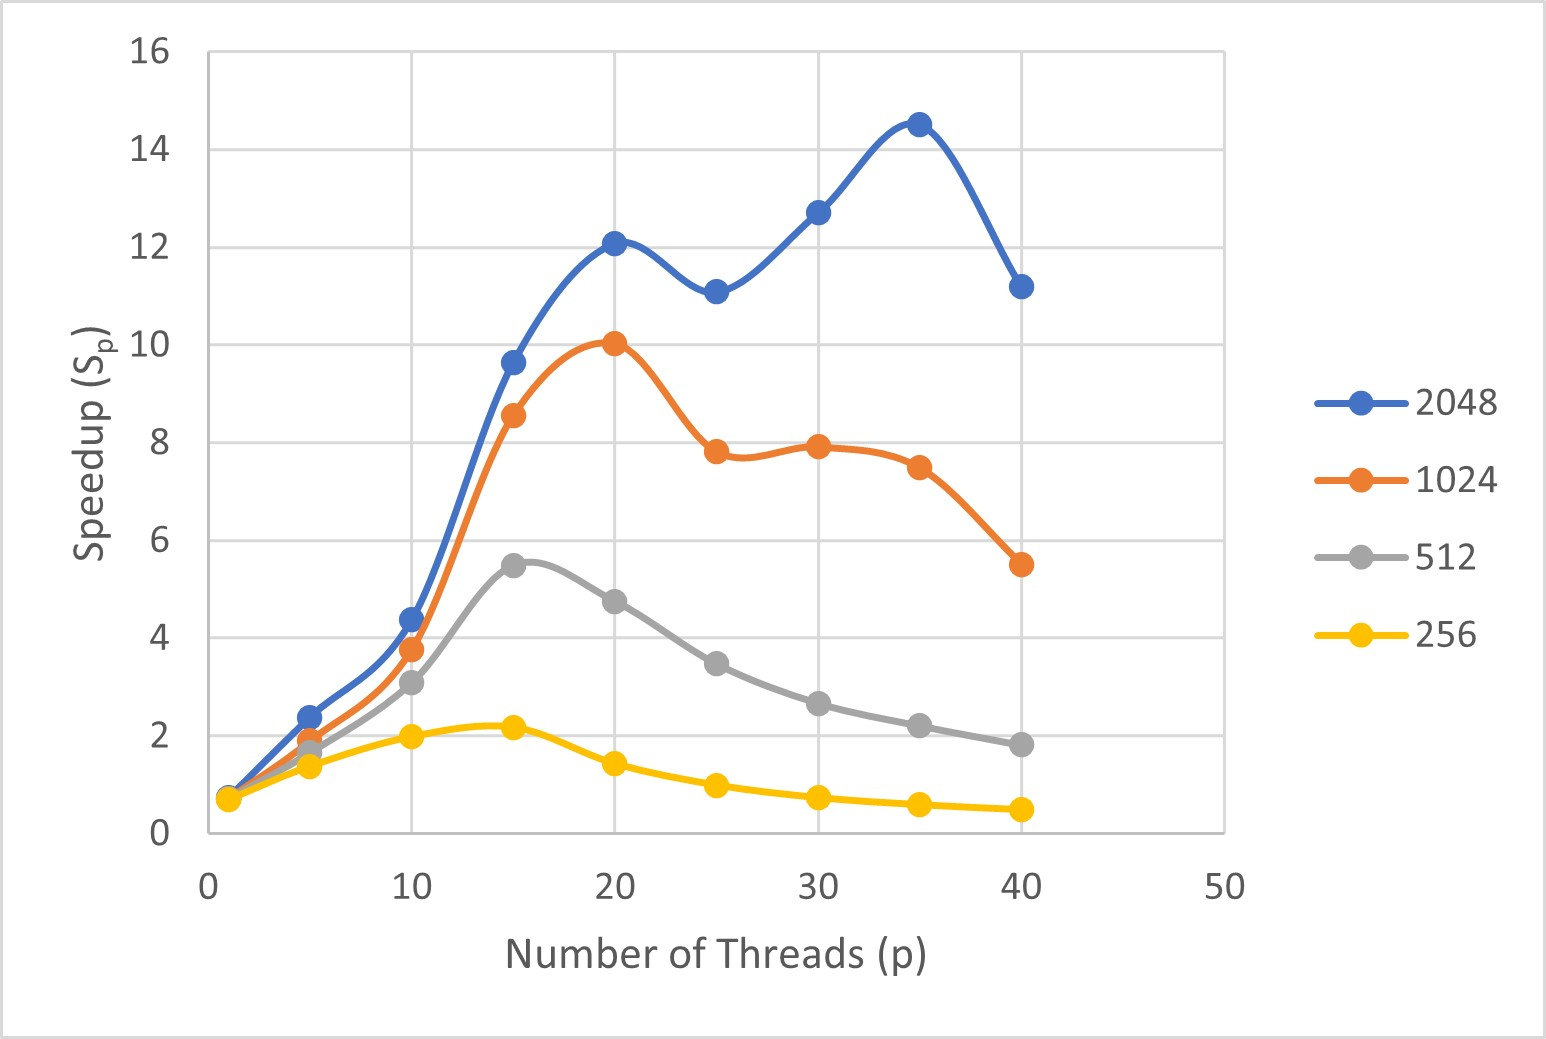
\includegraphics{Spscale}
    \caption{Graph of Speedup using $p$ threads for $n\in\{256, 512, 1024, 2048\}$}
    \label{fig:Spscale}
\end{figure}

Unfortunately, it was not possible to test $n=4096$, as the serial run exceeded the HPC cluster time limit of 20 minutes. Expectation would be that for larger matrices, efficiency and speedup will increase, and Karp-Flatt will decrease.

\begin{figure}[H]
    \centering
    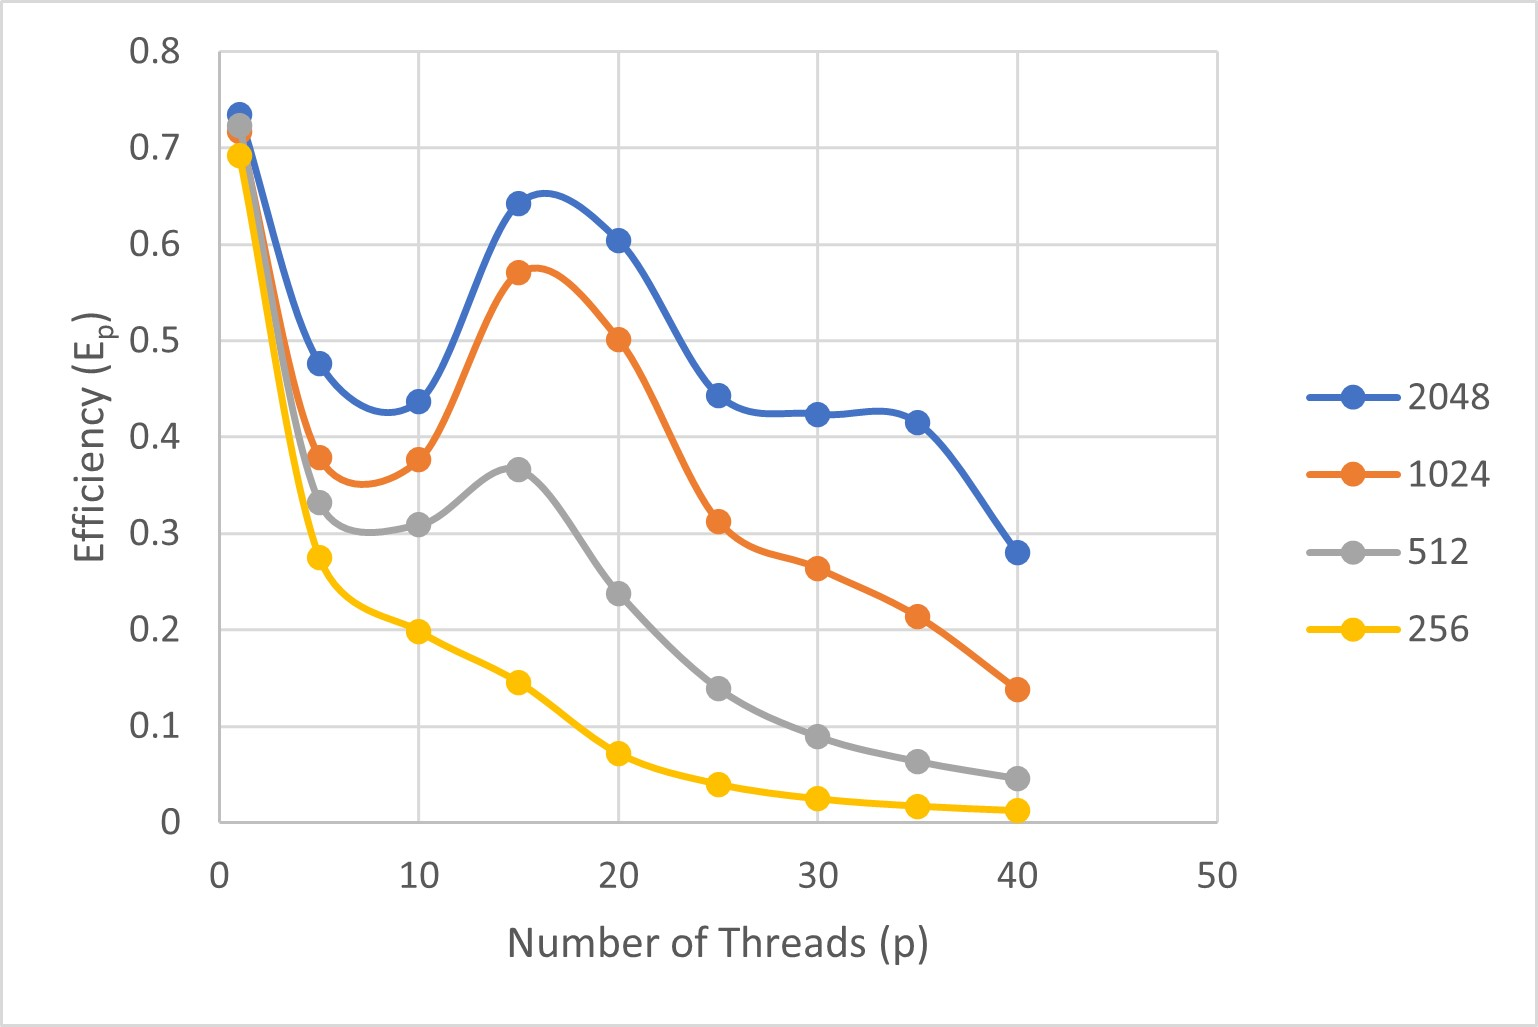
\includegraphics{Epscale}
    \caption{Graph of Efficiency using $p$ threads for $n\in\{256, 512, 1024, 2048\}$}
    \label{fig:Epscale}
\end{figure}

\begin{figure}[H]
    \centering
    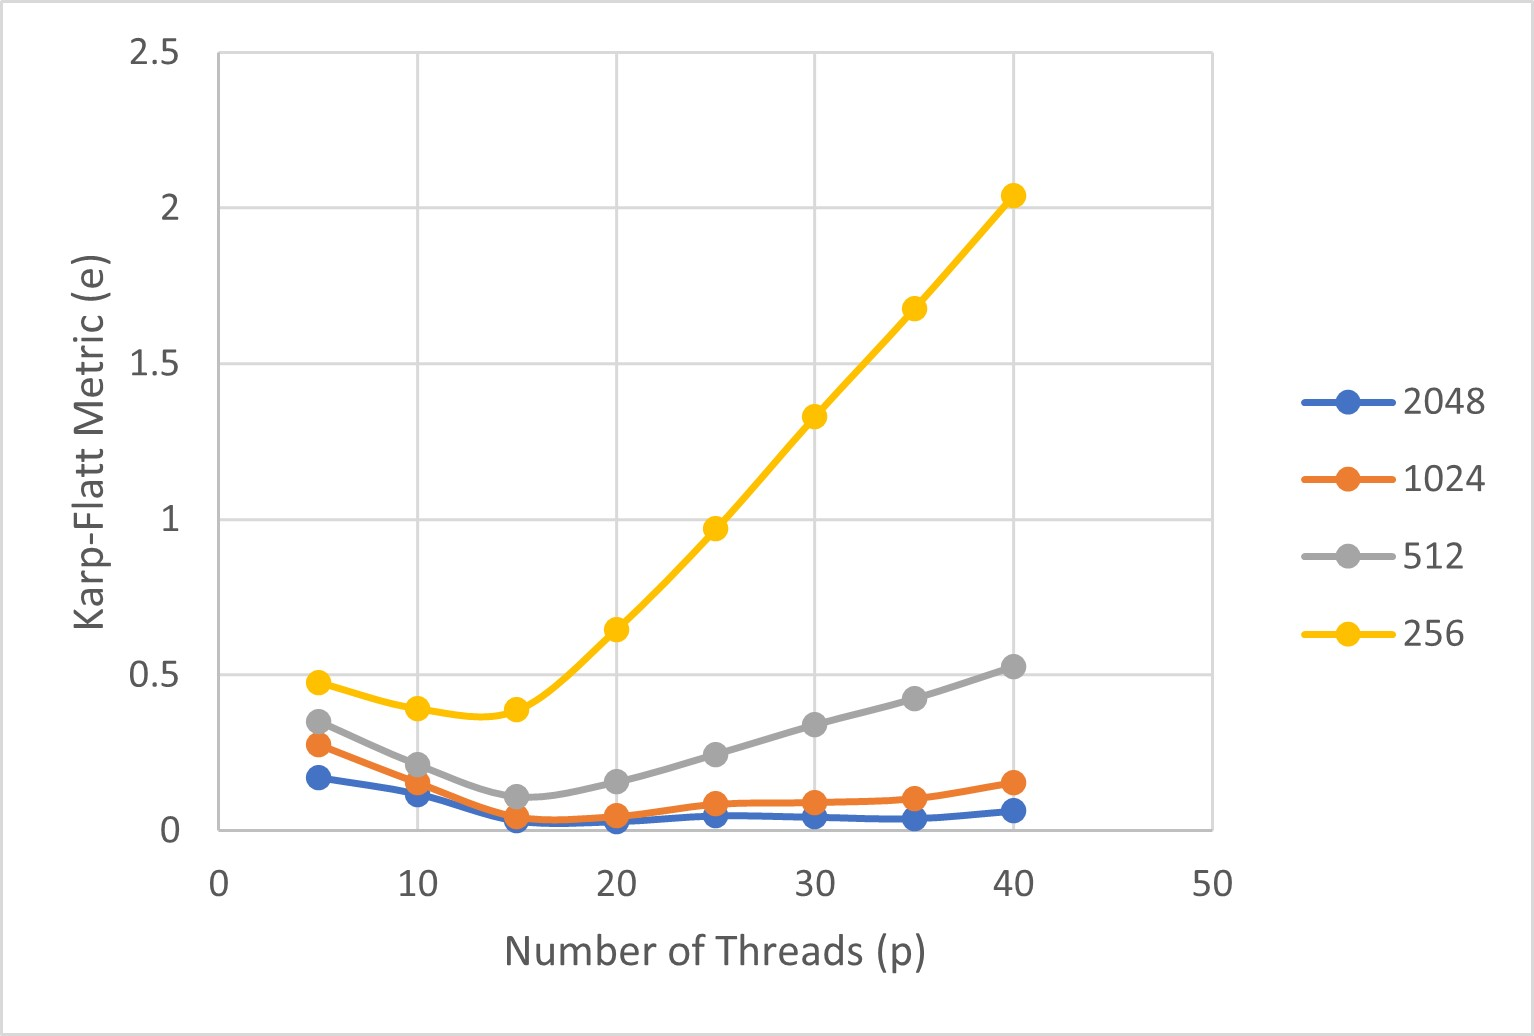
\includegraphics{kfscale}
    \caption{Graph of Karp-Flatt using $p$ threads for $n\in\{256, 512, 1024, 2048\}$}
    \label{fig:kfscale}
\end{figure}